\section{Adaptation realization}
\label{sec:adaptation}

% \cite{melenk2001} \cite{ainsworth1998} und so weiter

To indicate whetehr refinement or coarsening is going to happen by adding flags. Additionally, we want to set . Upon execution of refinement, the adaptation flags will we translated to \h-adaptation and all future fe indices will be considered as \p-adaptation.

But how do

Which finite element to pick on coarsened cells?

We found it to introduce so called \texttt{future fe indices} that determine the finite element that will be associated to its cell after refinement has happened.

We need to indicate which individual cell we will refine. Force p over h. Choose p over h.

This provides the basic functionality to \hp-adaptation on finite element data structures on distributed memory.


\begin{figure}
\begin{subfigure}{.5\textwidth}
  \centering
  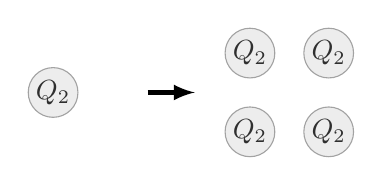
\begin{tikzpicture}[>=latex]
\def\Length{1}
\def\Radius{0.07}

% pre refinement
\LagrangeCell{0}{0}{2*\Length}{\Radius}{2}
  {{,,,,,,,,}};
\node[circle, draw=gray, fill=gray!20, inner sep=1pt, opacity=0.7, text opacity=0.8] at (\Length,\Length) {$Q_2$};

% arrow
\draw[->,ultra thick] (2.2*\Length,\Length) -- (2.8*\Length,\Length);

% post refinement
\LagrangeCell{3*\Length}{0}{\Length}{\Radius}{2}
  {{,,,,,,,,}};
\node[circle, draw=gray, fill=gray!20, inner sep=1pt, opacity=0.7, text opacity=0.8] at (3.5*\Length,0.5*\Length) {$Q_2$};

\LagrangeCell{4*\Length}{0}{\Length}{\Radius}{2}
  {{,,,,,,,,}};
\node[circle, draw=gray, fill=gray!20, inner sep=1pt, opacity=0.7, text opacity=0.8] at (4.5*\Length,0.5*\Length) {$Q_2$};

\LagrangeCell{3*\Length}{\Length}{\Length}{\Radius}{2}
  {{,,,,,,,,}};
\node[circle, draw=gray, fill=gray!20, inner sep=1pt, opacity=0.7, text opacity=0.8] at (3.5*\Length,1.5*\Length) {$Q_2$};

\LagrangeCell{4*\Length}{\Length}{\Length}{\Radius}{2}
  {{,,,,,,,,}};
\node[circle, draw=gray, fill=gray!20, inner sep=1pt, opacity=0.7, text opacity=0.8] at (4.5*\Length,1.5*\Length) {$Q_2$};
\end{tikzpicture}
  \caption{\hp-refinement.}
\end{subfigure}
\begin{subfigure}{.5\textwidth}
  \centering
  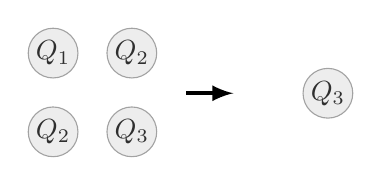
\begin{tikzpicture}[>=latex]
\def\Length{1}
\def\Radius{0.07}

% pre coarsening
\LagrangeCell{0}{0}{\Length}{\Radius}{2}
  {{,,,,,,,,}};
\node[circle, draw=gray, fill=gray!20, inner sep=1pt, opacity=0.7, text opacity=0.8] at (0.5\Length,0.5\Length) {$Q_2$};

\LagrangeCell{\Length}{0}{\Length}{\Radius}{3}
  {{,,,,,,,,,,,,,,,}};
\node[circle, draw=gray, fill=gray!20, inner sep=1pt, opacity=0.7, text opacity=0.8] at (1.5\Length,0.5\Length) {$Q_3$};

\LagrangeCell{0}{\Length}{\Length}{\Radius}{1}
  {{,,,}};
\node[circle, draw=gray, fill=gray!20, inner sep=1pt, opacity=0.7, text opacity=0.8] at (0.5\Length,1.5\Length) {$Q_1$};

\LagrangeCell{\Length}{\Length}{\Length}{\Radius}{2}
  {{,,,,,,,,}};
\node[circle, draw=gray, fill=gray!20, inner sep=1pt, opacity=0.7, text opacity=0.8] at (1.5\Length,1.5\Length) {$Q_2$};

% arrow
\draw[->,ultra thick] (2.2*\Length,\Length) -- (2.8*\Length,\Length);

% post coarsening
\LagrangeCell{3*\Length}{0}{2*\Length}{\Radius}{3}
  {{,,,,,,,,,,,,,,,}};
\node[circle, draw=gray, fill=gray!20, inner sep=1pt, opacity=0.7, text opacity=0.8] at (4*\Length,\Length) {$Q_3$};
\end{tikzpicture}
  \caption{\hp-coarsening.}
\end{subfigure}
\caption{Inheritance of cell characteristics through \hp-adaptation. We say $Q_1 \subset Q_2 \subset Q_3$.}
\label{fig:adaptation.}
\end{figure}